\tikzstyle{start} = [circle, inner sep = 0pt, opacity = 1]
\tikzstyle{end} = [circle, minimum width = 4pt, fill, inner sep = 1pt,
	opacity = 1]

\onslide<1->{
	\tikzstyle{endY} = [color = black, circle, minimum width = 4pt,
	    fill, inner sep = 1pt, opacity = 1]
	\tikzstyle{endG} = [color = black, circle, minimum width = 4pt,
	    fill, inner sep = 1pt, opacity = 1]
    \tikzstyle{edge} = [draw = black, opacity = 0]
    \tikzstyle{end7} = [circle, inner sep = 0pt, opacity = 0]
}
\only<6->{
  	\tikzstyle{endY} = [color = red, circle, minimum width = 4pt,
	    fill, inner sep = 1pt, opacity = 1]
    \tikzstyle{edge} = [draw = black, opacity = 1]
}

\only<7->{
  	\tikzstyle{endG} = [color = green, circle, minimum width = 4pt,
	    fill, inner sep = 1pt, opacity = 1]
    \tikzstyle{end7} = [circle, inner sep = 0pt, opacity = 1]
}
            
\tikzstyle{level 1} = [level distance = 0.1cm, sibling distance = 0.4cm]
\tikzstyle{level 2} = [level distance = 1.5cm]
\tikzstyle{level 3} = [level distance = 1cm]

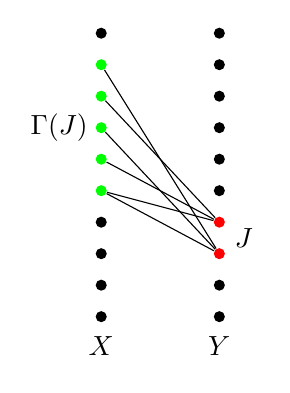
\begin{tikzpicture}[grow = right]
    \node [start]{}
    	child foreach \i in {10, 9}{
            node [end] (x\i) {}
               	child [end]{
	             	node [end] (y\i){}
    	            edge from parent [opacity = 0]
        	    }
            edge from parent [opacity = 0]
        }
        child foreach \i in {8, ..., 7}{
            node [end] (x\i) {}
               	child [endY]{
	             	node [endY] (y\i){}
    	            edge from parent [opacity = 0]
        	    }
            edge from parent [opacity = 0]
        }
        child foreach \i in {6, ..., 2}{
            node [endG] (x\i) {}
               	child [end]{
	             	node [end] (y\i){}
    	            edge from parent [opacity = 0]
        	    }
            edge from parent [opacity = 0]
        }
        child {
        	node [end] (x1) {}
           		child [end]{
	          		node [end] (y1){}
	    	        edge from parent [opacity = 0]
                }
    	   	edge from parent [opacity = 0]
        };

	\path [edge](y8) -- (x6);
    \path [edge](y8) -- (x4);
    \path [edge](y8) -- (x2);
    \path [edge](y7) -- (x3);
    \path [edge](y7) -- (x5);
    \path [edge](y7) -- (x6);

    \node at (x10.south) [below = 0.05cm] {$X$};
    \node at (y10.south) [below = 0.05cm] {$Y$};

    \path [opacity = 0](y7) -- (y8) node [start, midway] (mid){};
    \node <.(2)-> at (mid.east) [right = 0.05cm] {$J$};
    \node at (x4.west) [end7, left = 0.05cm] {$\Gamma(J)$};
\end{tikzpicture}